\documentclass[a4paper,landscape]{article}
\usepackage[margin=0mm,nohead,nofoot,nomarginpar]{geometry}
\usepackage{tikz}

% CONFIGURABLES
\def\linespacing{7}    % Spacing between lines
\def\gridspacing{7}    % Grid size
\def\dotspacing{7}     % Spacing between dots
\def\dotsize{0.5}      % Size of dots
\def\shadeval{20}      % Opacity percentage
\def\pagemargin{10}    % Page margin in mm
\def\startpage{1}      % Starting page number

% Calculate centering offset
\def\startx{0.25mm}

% Create A5 page content
\newcommand{\makepage}[4]{% #1=x-offset, #2=y-offset, #3=type, #4=page number
    \begin{scope}[shift={(#1,#2)}]
        % Page border (optional)
        \draw[black!10] (0,0) rectangle (148.5mm,210mm);

        % Content based on type
        \ifnum#3=1% Ruled
            % Title line
            \draw[black!\shadeval] 
                (\pagemargin mm,195mm) -- (138.5mm,195mm);
            % Regular lines
            \foreach \i in {1,...,25} {
                \draw[black!\shadeval] 
                    (\pagemargin mm,{195mm-\i*\linespacing mm}) -- 
                    (138.5mm,{195mm-\i*\linespacing mm});
            }
        \fi
        \ifnum#3=2% Grid
            \draw[step=\gridspacing mm,black!\shadeval] 
                (\pagemargin mm,15mm) grid (138.5mm,195mm);
        \fi
        \ifnum#3=3% Dots
            \foreach \x in {10,17,...,138} {
                \foreach \y in {15,22,...,195} {
                    \fill[black!\shadeval] (\x mm,\y mm) 
                        circle[radius=0.25mm];
                }
            }
        \fi

        % Page number - left or right based on position
        \ifdim#1<74mm % Left page
            \node[black!70] at (\pagemargin mm,7mm) {\small #4};
        \else % Right page
            \node[black!70] at (138.5mm,7mm) {\small #4};
        \fi
    \end{scope}
}

\begin{document}
\pagestyle{empty}

% Ruled pages
\noindent\begin{tikzpicture}[remember picture]
    \path[use as bounding box] (0,0) rectangle (297mm,210mm);
    \makepage{\startx}{0mm}{1}{\startpage}
    \makepage{148.75mm}{0mm}{1}{\the\numexpr\startpage+1}
\end{tikzpicture}
\newpage

% Grid pages
\noindent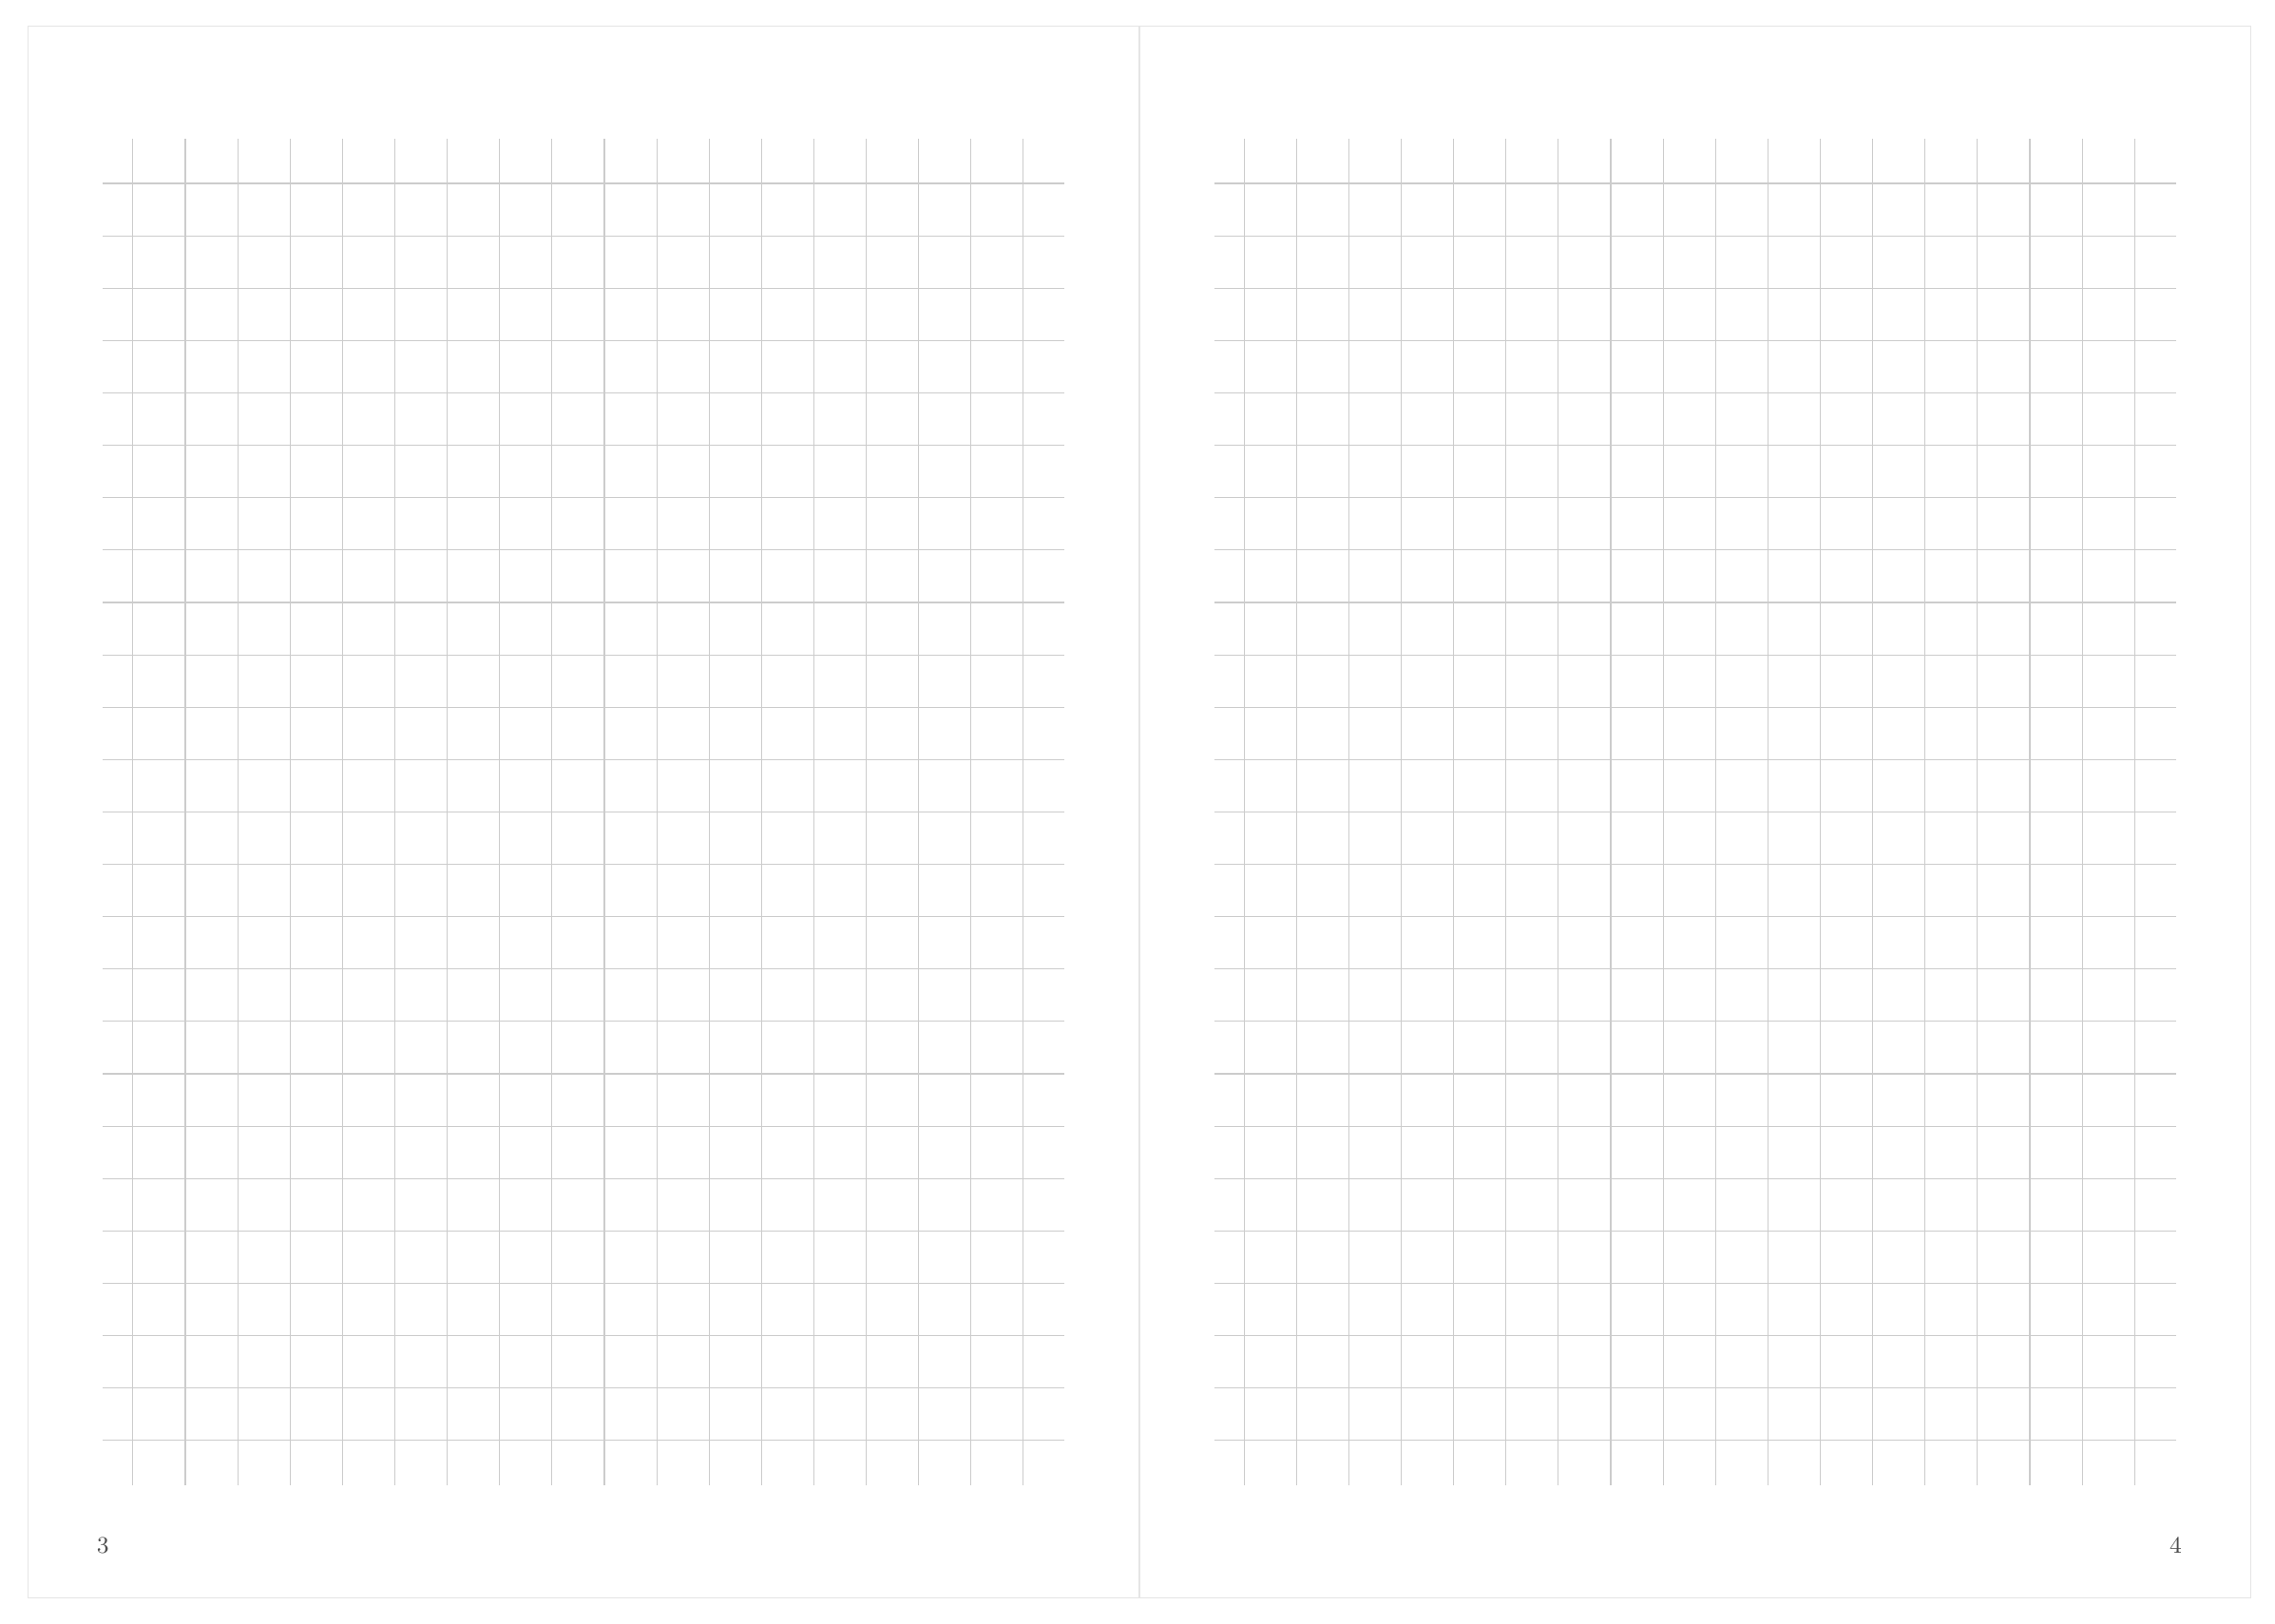
\begin{tikzpicture}[remember picture]
    \path[use as bounding box] (0,0) rectangle (297mm,210mm);
    \makepage{\startx}{0mm}{2}{\the\numexpr\startpage+2}
    \makepage{148.75mm}{0mm}{2}{\the\numexpr\startpage+3}
\end{tikzpicture}
\newpage

% Dot pages
\noindent\begin{tikzpicture}[remember picture]
    \path[use as bounding box] (0,0) rectangle (297mm,210mm);
    \makepage{\startx}{0mm}{3}{\the\numexpr\startpage+4}
    \makepage{148.75mm}{0mm}{3}{\the\numexpr\startpage+5}
\end{tikzpicture}

\end{document}
